\mode*		%% Reset Mode
\section{Getting Started}
\begin{frame}
	\frametitle{Installing Ti\emph{k}Z}

	Not necessary for \emph{new} TeXLive installs\ldots\\
	Sadly, this does not include School of CS Machines!

	\pause

	\begin{enumerate}
		\item Create a \texttt{texmf} directory
		\mode<article>
		\begin{itemize}
			\item \texttt{\$ mkdir \textasciitilde/texmf/}
		\end{itemize}
		\mode<all>

		\pause

		\item Download the PGF/Ti\emph{k}Z package
		\mode<article>
		\begin{itemize}
			\item Available from SourceForge \url{http://sourceforge.net/projects/pgf/}
		\end{itemize}
		\mode<all>

		\pause

		\item Extract the package in \texttt{\ldots/texmf/}

		\pause

		\item Run \texttt{texhash}
	\end{enumerate}
\end{frame}

\textit{Perhaps we should petition CSIS to get TikZ installed everywhere?}

\begin{frame}
	\frametitle{Using Ti\emph{k}Z}
	\begin{itemize}
		\item Include \texttt{\textbackslash usepackage\{tikz\}} in your \textit{preamble}
		\item Place Ti\emph{k}Z commands in the \texttt{tikzpicture} environment
	\end{itemize}
	\lstinputlisting[language=TeX]{examples.all/document.tex}
\end{frame}

\subsection{Drawing and Nodes}
\begin{frame}
	\frametitle{Drawing Primitives}
	Ti\emph{k}Z provides three drawing primitives:
	\begin{enumerate}
		\foreach \p in {path, draw, fill}{%
			\item \texttt{\textbackslash\p~[\textit{options}] \textit{co-ordinates};}
		}
	\end{enumerate}

	And three co-ordinate systems:
	\begin{description}
		\item[Cartesian] \texttt{(x \textit{units}, y \textit{units})}
		\item[Polar] \texttt{(angle in degrees:magnitude \textit{units})}
		\item[Named] \texttt{(predefined arbitrary name)}
	\end{description}
\end{frame}

This seems like the logical point to actually write some Ti\emph{k}Z, so we'll use each of the drawing primitives to draw a unit rectangle.
Along the way, we'll see what some of these mysterious options are.
The code used is shown in Listings \ref{listing.drawing-primitives.path}, \ref{listing.drawing-primitives.draw}, \ref{listing.drawing-primitives.fill};
and the results are in Figure \ref{figure.drawing-primitives}.

\begin{figure}[hb]
	\centering
	\foreach \primitive in {path, draw, fill}{%
		\begin{subfigure}{.25\textwidth}
			\centering
			\input{examples.article/drawing-primitives-\primitive}
			\caption{Drawing using ``\primitive''}
		\end{subfigure}
	}
	\caption{Using the TikZ drawing primitives to draw unit rectangles. Each primitive has its own unique quirks,
		and even though they are for the most part interchangeable, it's worth knowing what they are:
		namely, ``path'' will not display anything by default, so it can be quite useful for positioning nodes (more on this later);
		``fill'' will use the given colour to fill the area;
		and finally ``draw'' will use the given colour to stroke the area (I find I use this most).}
	\label{figure.drawing-primitives}
\end{figure}

\foreach \primitive in {path, draw, fill}{%
	\lstinputlisting[language=tex, caption={Using ``\primitive'' to draw}, label=listing.drawing-primitives.\primitive]%
		{examples.article/drawing-primitives-\primitive.tex}
}

\begin{frame}
	\frametitle{Shapes and Lines}
	We've seen the syntax for drawing rectangles, there's more\ldots
	\begin{description}
		\item[Rectangle] \texttt{rectangle (corner)} \tikz\draw [thick, red] rectangle (1em, 1em);
		\item[Circle] \texttt{circle [\textit{options}]} \tikz\draw [thick, blue] circle [radius=0.5em];
		\item[Ellipse] \texttt{ellipse [\textit{options}]} \tikz\draw [thick, purple] ellipse [x radius=.75em, y radius=.5em];
		\item[Curved Lines] \texttt{.. controls (-) and (-) ..}
			\tikz\draw [thick, green!50!black] (0,0)
				.. controls ++(0:0.5em) and ++(0:-0.5em) .. ++(1em, 1em)
				.. controls ++(270:.5em) and ++(0:-.5em) .. ++(.5em,-1em)
			;
		\item[Arcs] \texttt{arc [\textit{options}]} \tikz\draw [thick, gray] (0,0) arc [radius=1em, start angle=45, end angle=135];
	\end{description}
\end{frame}

Some further examples of these constructions are shown in Figure \ref{figure.drawing-primitives.shapes}, the code for which is shown in Listing \ref{listing.drawing-primitives.shapes}.

\begin{figure}[hbt]
	\centering
	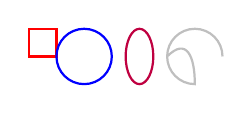
\begin{tikzpicture}
	%% Rectangle
	\draw [thick, red] (0,0) rectangle ++(1em, 1em);

	%% Circle
	\draw [thick, blue] (2em,0) circle [radius=1em];

	%% Ellipse
	\draw [thick, purple] (4em,0) ellipse [x radius=0.5em, y radius=1em];

	%% Curved Line linking into Arc
	\draw [thick, black!25!white] (5em,0)
		.. controls ++(45:1em) and ++(90:1em) ..
		++(1em,-1em) arc [start angle=270, end angle=0, radius=1em]
	;
	%% colour1!(0 <= x <= 100)!colour2 mixes colours by percentage
	%% i.e. black!25!white is 25% black, 75% white
\end{tikzpicture}

	\caption{Some more complicated constructions using TikZ drawing primitives.}
	\label{figure.drawing-primitives.shapes}
\end{figure}

\lstinputlisting[language=TeX, caption={More complicated shapes in TikZ}, label={listing.drawing-primitives.shapes}]{examples.article/drawing-primitives-shapes.tex}

\begin{frame}
	\frametitle{Nodes and Text}
	Amongst other things, nodes provide a way of adding text to a diagram.
	
	\texttt{\textbackslash node~\textit{at (...)} [\textit{options}] \textit{(name)} \{\textit{content}\};}

	\begin{center}
		\foreach \n in {1,...,4}{%
			\only<\n>{\input{examples.all/nodes-hello-\n}}
		}
	\end{center}

	\foreach \n in {1,...,4}{%
		\only<\n>{\lstinputlisting[language=tex]{examples.all/nodes-hello-\n.tex}}
	}

\end{frame}

\begin{frame}
	\frametitle{Nodes, Anchors and Co-ordinates}
	Nodes also provide our arbitrary co-ordinates/points.
	\begin{center}
		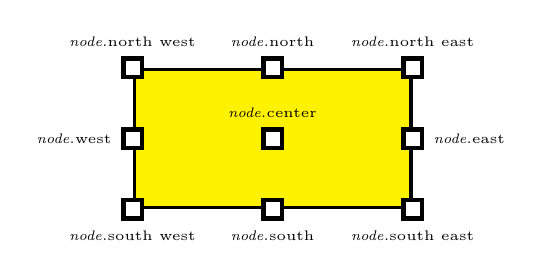
\begin{tikzpicture}[
	every label/.style = {font=\tiny},
]
	\node [minimum width=10em, minimum height=5em, draw, very thick, fill=yellow] (n1) {};

	\foreach \anchor/\labeldir in {west/left, north west/above, north/above, north east/above,
				       east/right, south east/below, south/below, south west/below, center/above}{%
		\node at (n1.\anchor) [label={\labeldir:{\textit{node}.\anchor}}, draw, ultra thick, fill=white] {};
	}
\end{tikzpicture}

	\end{center}
\end{frame}

We can put what we've got so far together in a fairly simple example.
Listing \ref{listing.nodes} shows the code for Figure \ref{figure.nodes}.

\begin{figure}[btp]
	\centering
	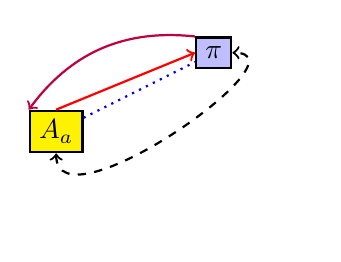
\begin{tikzpicture}
	%% Draw our two nodes -- note our content is mathematical
	\node at (0,0) [draw, thick, fill=yellow] (a) {$A_a$};		% Called `a'
	\node at (2,1) [draw, thick, fill=blue!25!white] (pi) {$\pi$};	% Called `pi'

	%% Connect up the node edges in various ways
	\draw [thick, dotted, blue] (a) -- (pi);	% Closest points
	\draw [thick, ->, red] (a.north) to (pi.west);	% `->' is an arrow
	\draw [thick, <->, dashed, out=-90, in=0] (a.south) to (pi.east); % Alternative bend mechanism
	\draw [thick, purple, bend left, <-] (a.north west) to (pi.north west);	% Yet another!
\end{tikzpicture}

	\caption{Uses of nodes and anchors; plus some additional options and semantic methods for constructing lines.}
	\label{figure.nodes}
\end{figure}

\lstinputlisting[language=TeX, caption={Combining nodes, anchors, and drawing.}, label={listing.nodes}]{examples.article/nodes-anchors.tex}

\mode<all>	%% Reset mode
